\chapter{Application development}
\lhead{Chapter 3 \emph{Application development}}
\label{chap:3}
%\autoref{chap:3}
\bigskip

The mitigation of the overpopulation problem is nowadays an absolute necessity. The application, which is described below, has been developed towards this direction. More specifically, it can give the incentives to create space traffic management rules based on the orbit and capacity allocation, as well as the added value that each new satellite has.

The application has two major capabilities. The first one is the calculation of the revisit time of a single satellite or constellation (Section \ref{revisit time}). The second one is a tool, with which the user can find out what is the added value of an object based on the number of the satellites that are already in-orbit and have the same characteristics (Section \ref{added value}). This tool, in essence, has many more capabilities, which are presented in Chapter 4.%\ref{chap:4}.

\bigskip
\section{From satellite definition to revisit time calculation}
\label{revisit time}
\bigskip

The implementation of this first part of the application was programmed and carried out in Python. In this stage, the user defines a satellite by providing its two-line elements (TLE). However, since the application is focused only on the Earth Observation satellites, parameters related to this field are also necessary to be given. Consequently, a number of steps need to be done in order to compute the orbit of the satellite: calculation of the polar coordinates in the orbital plane, the position that it has in the space-fixed system and later in the earth-fixed system and finally the calculation of the longitude and latitude on the Earth's surface.
%Write epigrammatika all the different steps here.

\bigskip
\subsection{Necessary input data}
\label{input_data}
\bigskip

In this first step, the user can define a satellite by providing the TLE set to the application. Despite the fact that the classical orbital elements are used in the scientific community, it was decided that the TLE set is a more convenient and fast way of importing and handling the input data, since the latter way is applied universally and the orbit computation in the next step can be done without any further conversions of those given parameters.

From the elements of a TLE set, eight parameters are being extracted and used in the application. Those are the epoch date, inclination ($i$), Right Ascension of the Ascending Node (RAAN) ($\Omega$), eccentricity ($e$), argument of perigee ($\omega$), mean anomaly ($M$), mean motion ($n$) and the international designator, which is a unique code of a satellite. In the Figure \ref{tle}, it can be seen an example dataset with all the information that TLE carries.

More specifically, the epoch date is the number of days passed in the particular year. The information about the year is taken from the first two digits of the parameter and from the following digits the exact month, day, epoch hour, minute and second can be found. Finally, the epoch time is calculated in seconds as:

\begin{equation}
\label{epoch}
\text{epoch} = (\text{epoch hour} * 3600) + (\text{epoch min} * 60) + \text{epoch sec}.
\end{equation}

\begin{figure}
\centering
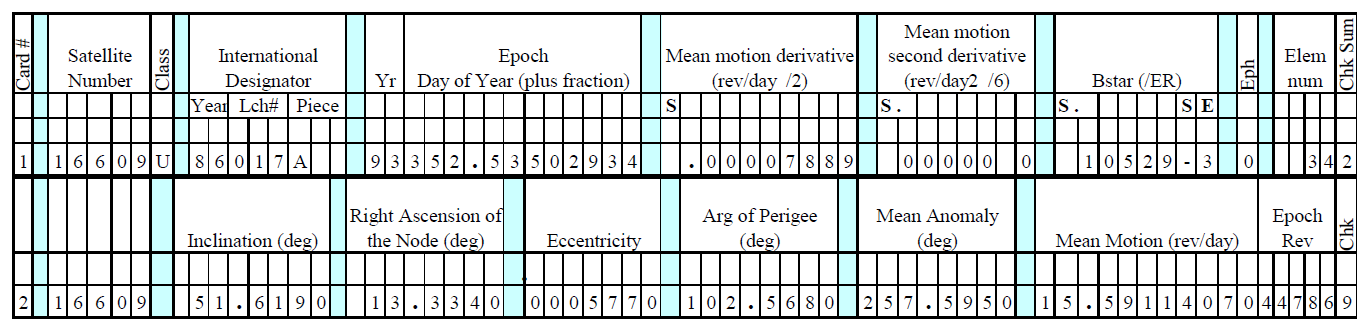
\includegraphics[width=0.9\textwidth]{Images/tle.png}\caption{An example two-line element (TLE) set. S is the sign of values, and E is of exponent. \textit{Source: \cite{Vallado}}}
\label{tle} 
\end{figure}

The parameters of eccentricity, inclination, RAAN, argument of perigee and mean anomaly can be seen graphically in the Figure \ref{keplerian_elements}. In short, eccentricity is a constant defining the shape of the orbit. There is a circular orbit when it is zero and an elliptical orbit when the number is less than one. To the given value of eccentricity from the TLE, a decimal at the beginning must be applied. As far as the inclination, which is given in degrees, it is the angle between the equator and the orbit plane. The RAAN or else the node (degrees) is the angle between vernal equinox and the point where the orbit crosses the equatorial plane and goes towards the north. Argument of perigee is the angle between the ascending node and the orbit's point of the closest approach to the earth, which is called perigee. It is given in degrees. Finally, the mean anomaly is the angle of satellite location in the nominal orbit, which referenced to a circular orbit with radius equal to the semi-major axis. It is measured from the perigee and it is also given in degrees. It should be also noted that the conversion of their units from degrees to radians is necessary, since many other computations will be followed. \cite{Vallado}

From the parameter of mean motion ($n$), the semi-major axis ($a$), as well as the period ($T$) of the orbit can be found. Namely, the mean motion is converted from the unit of $revolutions/day$ to $radian/sec$. Then, the semi-major axis is calculated from the Kepler's 3\textsuperscript{nd} law:
\begin{equation}
\label{3rd_keplers_law}
n^2 a^3 = \mu,
\end{equation}
%a = (\frac{\mu}{n^2})^{1/3},
with $\mu$ being the geometric gravitational parameter.

\begin{figure}
\centering
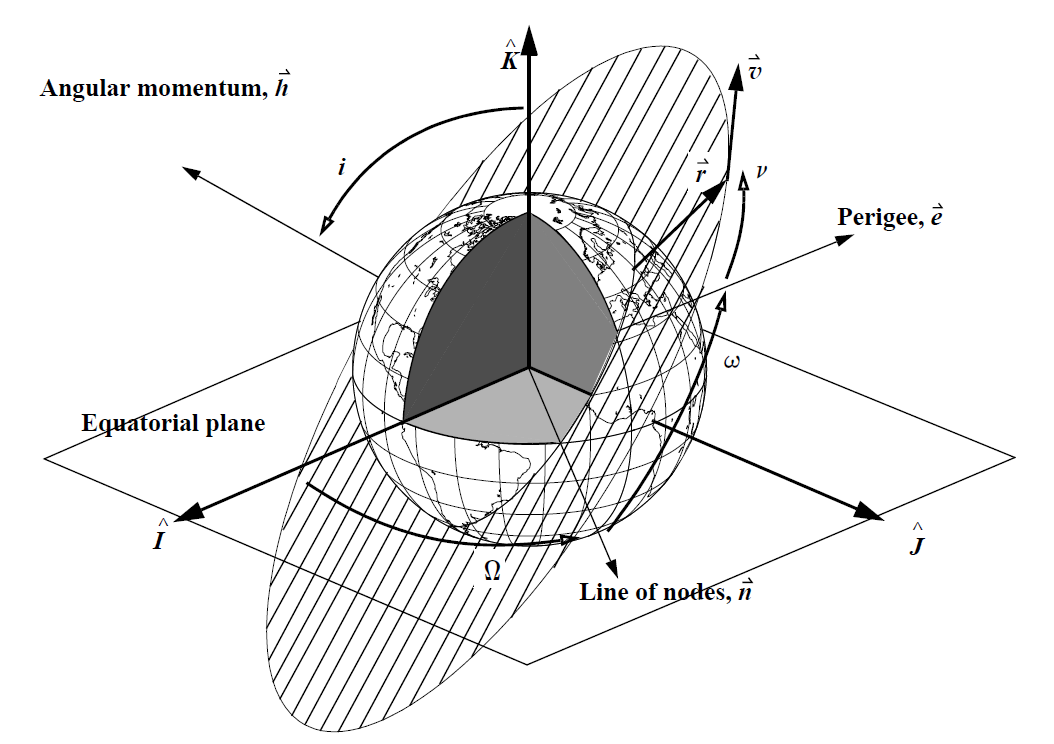
\includegraphics[width=0.9\textwidth]{Images/keplerian_elements.png}\caption{The classical orbital elements: semi-major axis ($a$), eccentricty ($e$), inclination ($i$), Right Ascension of the Ascending Node (RAAN) ($\Omega$), argument of perigee ($\omega$), and true anomaly ($\nu$). \textit{Source: \cite{Vallado}}}
\label{keplerian_elements} 
\end{figure}

Apart from the parameters that were just mentioned, it is necessary to be added some parameters related to the Earth Observation sensor that the satellite has. The orbit lifetime, the type of sensor (see Section \ref{EO}) and the spatial resolution are some of them. However, the determiner parameter in the calculation of the revisit time is the information of the swath width of the sensor, which is inserted in the units of kilometers. Swath is called the area of the Earth that is captured on the image and thus the bigger the number of swath is, the larger the area that is captured. In the Figure \ref{swath_width}, both the swath width and the spatial resolution are illustrated. Those parameters are usually inversely proportional; the higher spatial resolution, the less area is covered by a single image and thus the smaller the swath width.

\begin{figure}
\centering
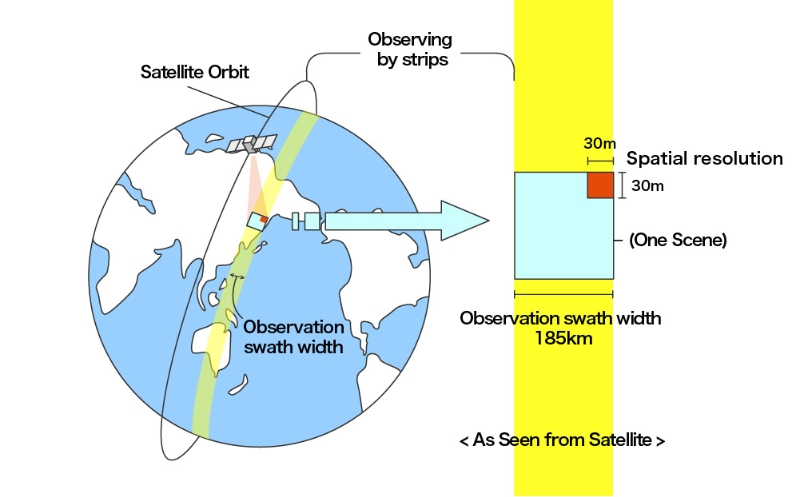
\includegraphics[width=0.9\textwidth]{Images/swath_width.png}\caption{Illustration showing the difference between swath width and spatial resolution. \textit{Source: Remote Sensing Technology Center of Japan - EO in Japan. Website: restec.or.jp (Accessed: October, 2020)}} %https://www.restec.or.jp/en/knowledge/sensing/sensing-3.html
\label{swath_width} 
\end{figure}

\bigskip
\subsection{Orbit computation}
\bigskip

The next step is the computation of the orbit. The imported parameters are given in a geocentric reference system and they define a unique orbit.

\bigskip
\subsubsection{Polar coordinates in orbital plane}
\bigskip

Firstly, the polar coordinates, which are the radius ($r$) and the true anomaly ($v$) are calculated. For this calculation though, the eccentric anomaly ($E$) needs to be found through this transcendental Kepler's equation:
\begin{equation}
E - e \sin{E} = M,
\end{equation}

where $M$ is the mean anomaly. Once the equation has be solved iteratively, the radius ($r$) and true anomaly ($v$) can be found.
\begin{equation}
r = a(1 - e \cos{E}),
\end{equation}

\begin{equation}
\tan{\frac{\nu}{2}} = \sqrt{\frac{1 + e}{1 - e}} \tan{\frac{E}{2}}.
\end{equation}

\bigskip
\subsubsection{Position \& velocity in space-fixed system}
\bigskip

The main idea of this task is the rotation of the orbital plane into the equatorial coordinate system. The angles that were used to the rotation matrices were the RAAN ($\Omega$), the inclination ($i$), and the argument of perigee ($\omega$). In the Figure \ref{orbit_to_space}, the rotation of the orbital plane is illustrated based on the aforementioned angles. For achieving that, the position (Equation \ref{position_orbital}) and velocity (Equation \ref{velocity_orbital}) in the orbital plane should be calculated first \cite{Montenbruck}:

\begin{figure}
\centering
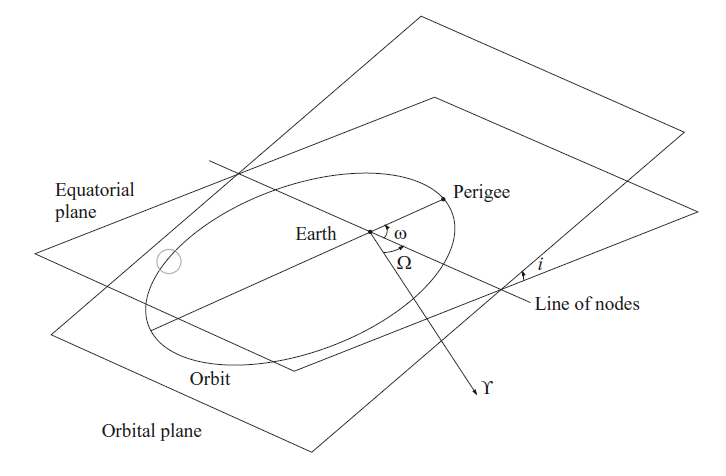
\includegraphics[width=0.9\textwidth]{Images/orbit_to_space.png}\caption{The rotation of the orbital plane into the equatorial plane with the help of the following orbital elements of the satellite: inclination ($i$), RAAN ($\Omega$) and argument of perigee ($\omega$). \textit{Source: \cite{Montenbruck}}}
\label{orbit_to_space} 
\end{figure}

\begin{equation}
\label{position_orbital}
\vv{r_{b}} = r \begin{bmatrix} \cos{v} \\ \sin{v} \\ 0 \end{bmatrix}
\end{equation}
\begin{equation}
\label{velocity_orbital}
\dot{\vv{r_{b}}} = \sqrt{\frac{\mu}{a (1 - e^2)}} \begin{bmatrix} -\sin{v} \\ e + \cos{v} \\ 0 \end{bmatrix},
\end{equation}

where $\mu$ the geometric gravitational parameter (Equation \ref{3rd_keplers_law}).

Then, the position and the velocity in the space-fixed system are found through \cite{Montenbruck}:
\begin{equation}
\label{space-fixed}
\vv{r} = R_3 (-\Omega) R_1  (-i) R_3 (-\omega) \vv{r_{b}},
\end{equation}
\begin{equation}
\dot{\vv{r}} = R_3 (-\Omega) R_1  (-i) R_3 (-\omega) \dot{\vv{r_{b}}},
\end{equation}
where $\vv{r_{b}}$, $\dot{\vv{r_{b}}}$ are taken from the equations \ref{position_orbital}, \ref{velocity_orbital} respectively. The elementary matrices that were used are:
\begin{equation}
R_1(\theta) = \begin{bmatrix} 1 & 0 & 0 \\ 0 & \cos{\theta} & \sin{\theta} \\ 0 & -\sin{\theta} & \cos{\theta} \end{bmatrix},
\end{equation}
for the rotation around the x-axis ($R_{1}$), and
\begin{equation}
\label{R3}
R_3(\theta) = \begin{bmatrix} \cos{\theta} & \sin{\theta} & 0 \\ -\sin{\theta} & \cos{\theta} & 0 \\ 0 & 0 & 1 \end{bmatrix},
\end{equation}
for the rotation around z-axis ($R_{3}$) \cite{Montenbruck}.

\bigskip
\subsubsection{Position \& velocity in earth-fixed system}
\bigskip

After the orbit calculation in the space-fixed system, the position and velocity in the earth-fixed system can be found. Based on the rotation rate of the Earth ($\Omega_{E}$) and the sidereal angle, the angle of rotation ($\theta_{0}$) (Equation \ref{theta_angle}) between the space and earth system is calculated. The sidereal angle is calculated through the Greenwich mean sidereal time \cite{Vallado}, having as an input the Julian date from the information about the epoch time (Equation \ref{epoch}).

\begin{equation}
\label{rotation_rate}
\Omega_{E} = \frac{2 \pi}{86164}
\end{equation}

\begin{equation}
\label{theta_angle}
\theta_{0}(t) = \Omega_{E} \cdot t + \text{sidereal angle}
\end{equation}

Both angles, the angle of rotation $\theta_{0}$ and the sidereal angle, should be in radian in order to be used in the following steps. Finally, the position in the earth-fixed system is calculated using the rotation matrix around the z-axis (Equation \ref{R3}) as:
\begin{equation}
\vv{r}_{Earth-fixed}(t) = R_{3}(\theta_{0}(t)) \vv{r},
\end{equation}
where $\vv{r}$ is the position in the space-fixed system (Equation \ref{space-fixed}).

\bigskip
\subsubsection{Longitude \& latitude on the Earth's surface}
\bigskip

In order to calculate the position of the sub-satellite's points on the Earth's surface, the longitude and latitude is needed. The equations that link the Earth-fixed coordinates with the $\lambda$ and $\phi$ are the following:

\begin{equation}
\tan{\lambda} = \frac{y_{\text{Earth-fixed}}}{x_{\text{Earth-fixed}}},
\end{equation}

\begin{equation}
\tan{\phi} = \frac{z_{\text{Earth-fixed}}}{\sqrt{x^2_{\text{Earth-fixed}} + y^2_{\text{Earth-fixed}}}}.
\end{equation}

The groundtrack of the orbit, which is the path of the sub-satellite point as the satellite travels through its orbit, can be consequently acquired. However, the actual groundtrack of a satellite differs from a simple circle that results from the intersection of the orbital plane with the surface of the Earth. For a satellite with a period $T$, the longitude $\lambda$ is shifted from one revolution to the next \cite{Montenbruck} :
\begin{equation}
\Delta \lambda_{\Omega} = - \dot{\theta} \cdot T = - 0.2507^{\circ}/ min \cdot T,
\end{equation}

where $\dot{\theta}$ is the Greenwich mean sidereal at time $t$. This is due to the Earth's rotation, as it can be seen in the Figure \ref{groundtrack-fixed-rotating}.

\begin{figure}
\centering
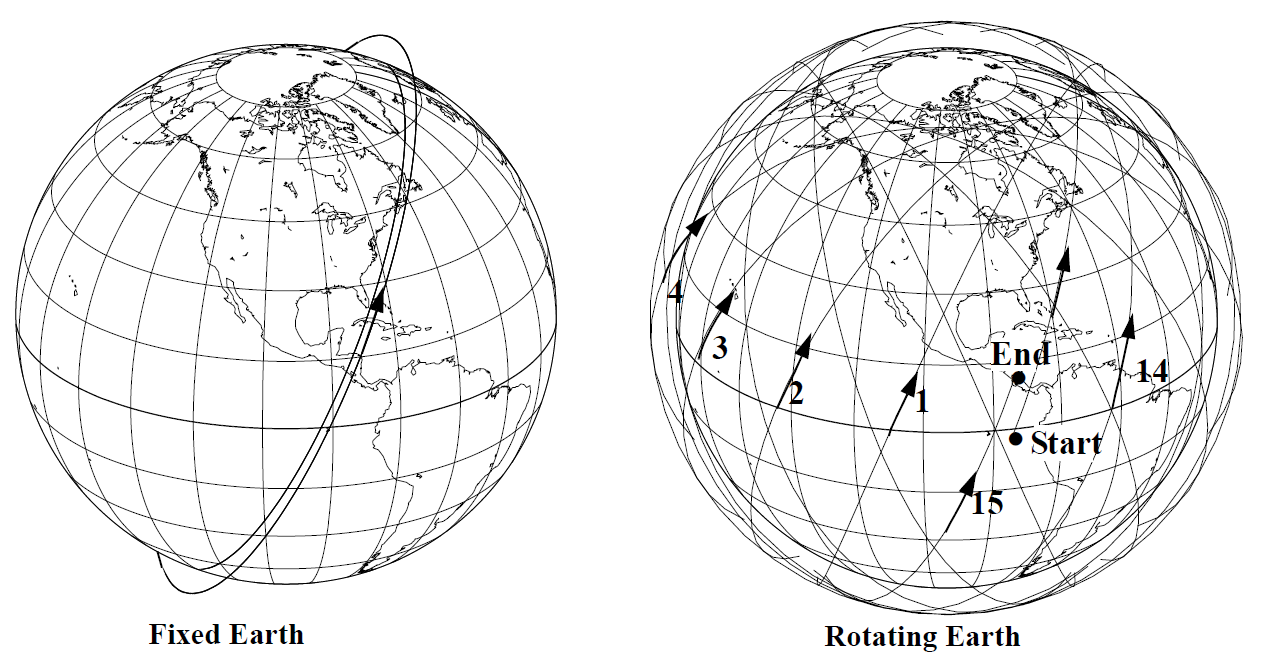
\includegraphics[width=0.9\textwidth]{Images/groundtrack-fixed-rotating.png}\caption{Illustration of the groundtracks in cases where the Earth is fixed and rotating. \textit{Source: \cite{Vallado}}}
\label{groundtrack-fixed-rotating} 
\end{figure}

\bigskip
\subsubsection{Perturbation on the orbital elements}
\bigskip

Since the focus of this application is on the low earth orbit (LEO) satellites, the gravity field is the largest perturbation, which cause secular motion to some of the orbital elements. The RAAN is one the affected by the zonal harmonics, and the equation that describes it:
\begin{equation}
\dot{\Omega} = - \frac{3 n R_{\bigoplus}^{2} J_{2} \cos{i}}{2 a^{2}},
\end{equation}
where $R_{\bigoplus}$ is the radius of the Earth according to WGS-84 (6378.137 km), and as $n$ the mean motion is used \cite{Montenbruck}.

Due to secular perturbations, the argument of perigee is also affected:
\begin{equation}
\dot{\omega} = - \frac{3 n R_{\bigoplus}^{2} J_{2}}{4 a^{2}} (1 - 5 \cos^{2}{i}).
\end{equation}

% Vallado p. 674 + Montenbruck p.50

\bigskip
\subsubsection{Revisit time definition}
\bigskip

The goal of the first part of the application is to find the revisit time of the satellite. Thus, its definition needs to be noted. The revisit time is the time elapsed between two successive observations of the same ground point on the surface of the Earth. \cite{Luo} To be more specific, since this application will produce one number as the revisit time of a satellite, this number refers to the average revisit time of all the ground points in the equator. However, the user has the capability of inserting in the application a latitude, in which he/she is interested in knowing the revisit time, other than the one in the equator which comes by default. More elaborated description regarding its calculation is being followed.

%ABOUT REVISIT TIME:
%The interval of time required for the satellite to complete its orbit cycle is not the same as the "revisit period". Due to the steerable sensors, the off-nadir angles, the large swath width , the revisit time can be less than the orbit cycle time. "The revisit period is an important consideration for a number of monitoring applications, especially when frequent imaging is required (for example, to monitor the spread of an oil spill, or the extent of flooding). In near-polar orbits, areas at high latitudes will be imaged more frequently than the equatorial zone due to the increasing overlap in adjacent swaths as the orbit paths come closer together near the poles." (Source: https://www.nrcan.gc.ca/maps-tools-and-publications/satellite-imagery-and-air-photos/remote-sensing-tutorials/acknowledgements-permission-use/9391)

\bigskip
\subsection{Computational calculation of revisit time}
\bigskip

One key element needed in order to calculate the revisit time is the observation swath width, or the spatial extent or else the area that is captured on the ground by the satellite's sensor. This is an information that is already given, as stated in the Section \ref{input_data}, and this is the parameter of the swath width (see Figure \ref{swath_width}). Thus, taking into account the swath width, a grid in the global map can be created, which will be consisted of cells simulating the area on the ground that is captured by the satellite. The global map is represented as a two-dimensional map in comparison with a three-dimensional map, since the computations can be executed easier later.

\bigskip
\subsubsection{Map projection}
\bigskip

The map projection that was chosen is a equidistant cylindrical, which forms a grid of equal rectangles. In this projection the poles are represented as straight lines across the top and bottom of the grid, the same length as the equator line. It is worth mentioning that the distortion in the shape, scale and area increases as the distance from the equator increases. \cite{Lapaine} An example of this map projection is shown in Figure \ref{map_projection}, as it was generated by the Python code. The selection of this projection was made, since the distortions in the polar regions can be easily corrected, in comparison i.e. with a Mercator projection. The grid of equal rectangles resembles also an array in python, which makes the calculations more comprehensible.

\begin{figure}
\centering
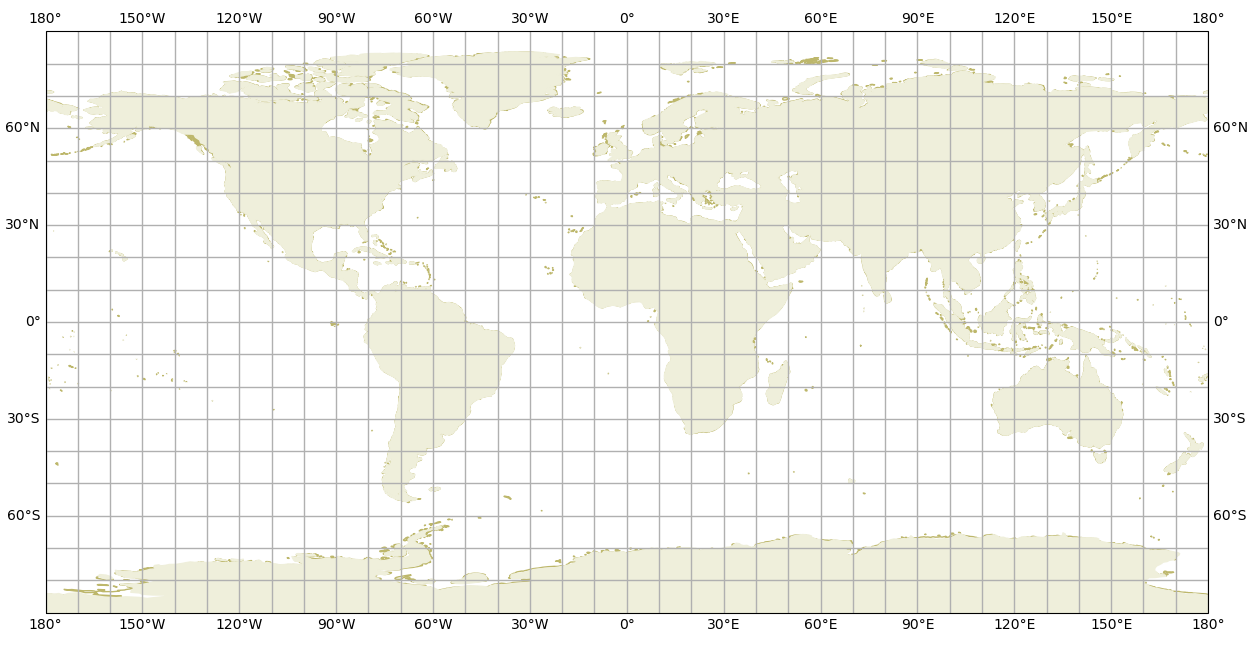
\includegraphics[width=0.9\textwidth]{Images/map_projection.png}\caption{A cylindrical equidistant map projection that was used in the application. It forms a grid of equal rectangles. \textit{Source: Python code}}
\label{map_projection}
\end{figure}

\bigskip
\subsubsection{Grid creation}
\bigskip

The grid that is created on the global map is consisted of cells, whose size is the same as the swath width that is captured by the sensor of the satellite. Since the global map handles geographic degrees, 360 degrees in the longitude and 180 degrees in the latitude, the swath width needs to be converted as it was given originally in the unit of kilometers. A rule of thumb in the conversion is that 111 kilometers are approximately 1 degree. Thus, the interval between the cells, which is also named as grid interval in this application, can be found from the equation:
\begin{equation}
\label{grid_interval}
\text{grid interval} = \text{swath width} \cdot 0.008
\end{equation}

Considering that the grid interval is known (Equation \ref{grid_interval}), the number of the cells that can fit in the global map is found. An important feature in the creation of the grid is that the zero degree latitude and longitude is always included in a cell (Figure \ref{map_projection_0covered}). In the case of a satellite with zero inclination, whose viewing latitudes are mostly the equatorial ones, cells containing the zero degree latitude are the ones apparently revealing the information about the revisit time in those regions. So in those cases, cells including the zero latitude are of utmost importance. However, this application focuses on Earth Observation (EO) satellites in the LEO region, whose orbits are usually near-polar. Hence, this feature can be truly beneficial when equatorial or tropical orbits are imported to the application.

\begin{figure}
\centering
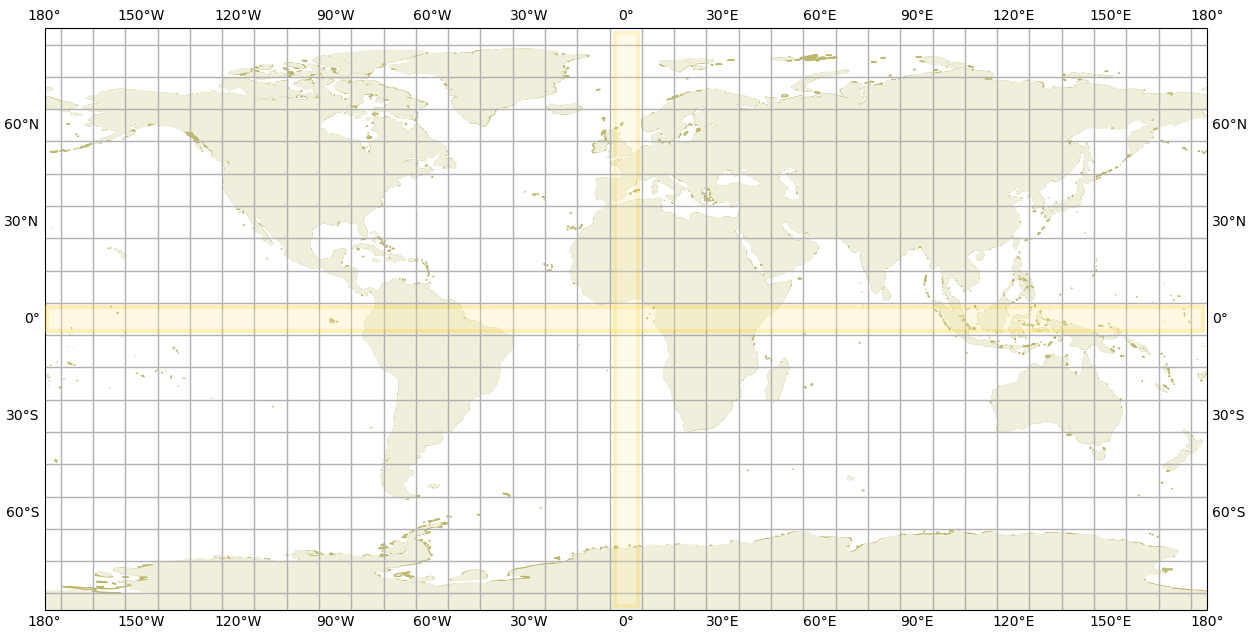
\includegraphics[width=0.9\textwidth]{Images/map_projection_0covered.png}\caption{The zero longitude and latitude is always centered to a grid's cell. \textit{Source: Python code}}
\label{map_projection_0covered}
\end{figure}

\bigskip
\subsubsection{Correction of map distortion}
\label{Correction of map distortion}
\bigskip

As it was mentioned before, the map projection that is used, exhibits distortions, which increase the further the place is located from the equator. This happens due to the fact that the poles are represented as straight lines, which are parallel and have the same length as the equatorial line. An example of how the swath width of a satellite seems to increase as the satellite moves towards the poles can be seen in Figure \ref{distortion_show-swath-width}. All the same, the swath width of the satellite's sensor remain constant throughout its orbit.

\begin{figure}
\centering
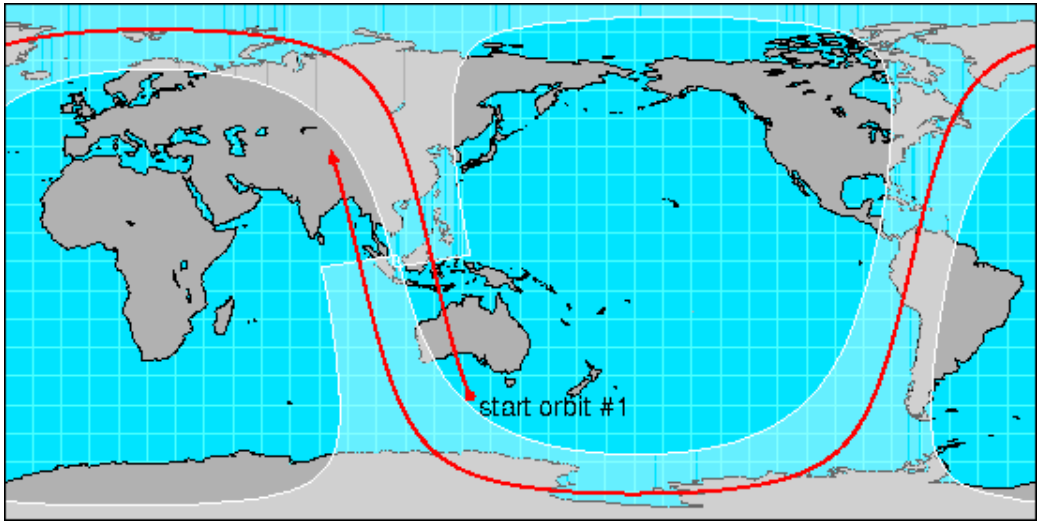
\includegraphics[width=0.9\textwidth]{Images/distortion_show-swath-width.png}\caption{A near-polar orbit illustration of a sun-synchronous meteorological satellite. Its instrument scans approximately 3000 km wide swath. Due to the map distortion, the viewing area seems to be larger when the satellite passes closer to the poles. \textit{Source: National Center for Atmospheric Research, Boulder, Colorado, USA. Url: ral.ucar.edu/~djohnson/satellite/coverage.html (Accessed September 30, 2020)}}
\label{distortion_show-swath-width}
\end{figure}

For the correction due to the map distortion, the simple assumption of a spherical Earth has been made. Then, it has been assumed, that the equator's length is 360 degrees, whereas the meridians of the Earth intersect on the poles, leading to a point (zero length) in the poles. As it can be seen in Figure \ref{correction_map_distortion}, the hypotenuse of the illustrated triangle is found using the Pythagorean theorem, and based on this side, the angle $\phi$ is found from: $$ \cos{\phi} = \frac{90}{\text{hypotenuse}}.$$
Thus, based on the $\phi$ angle (constant) and the latitude of the sub-satellite point, a swath width depicting the area that the satellite is actually scans, is calculated. In this way, the distortion is corrected.

\begin{figure}
\centering
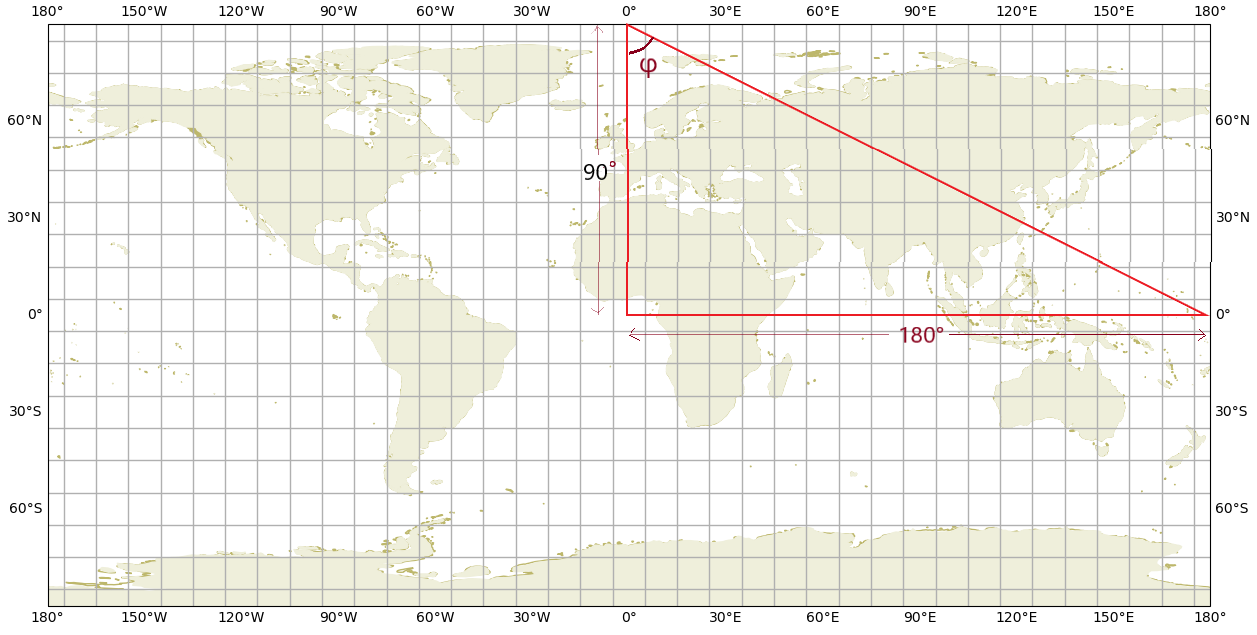
\includegraphics[width=0.9\textwidth]{Images/correction_map_distortion.png}\caption{The triangle shows the approximation method of correcting the distortion of the map. The poles instead of having a 360 degrees length, are assumed to be points. \textit{Source: Python code}}
\label{correction_map_distortion}
\end{figure}

\bigskip
\subsubsection{Space-time sampling of the satellite}
\bigskip

Before the actual procedure of counting cells starts, it should be assured that the interval between the sub-satellite points will give enough information for the revisit time calculation. To be more specific, during the orbit that is depicted in the groundtrack, there should not be empty cells neither too many points on the same area, so that it seems that the satellite has passed more than one times. This so-called space-time sampling in the LEO satellites is dependent on the orbit. For this reason, the height of the satellite should be considered. The height of the satellite is given through the semi-major axis $a$, which is connected with the mean motion $n$ through the equation \ref{3rd_keplers_law}. From the equation: $$n = \frac{2 \pi}{T}, $$
the information of the period $T$ is found, with which the interval between the points can be calculated. It is a fact that in one orbit (one period) the satellite passes above 360 degrees, as it can be seen in Figure \ref{ascending-descending} showing the groundtrack of Sentinel-2A. Then, the unknown time interval can be found through the equation:
\begin{equation}
\text{interval} = \frac{\text{grid interval} \cdot T}{360}
\end{equation}

since the grid interval is known (equation \ref{grid_interval}).

\bigskip
\subsubsection{Tracking of satellite's path}
\bigskip

The calculation of the revisit time is actualized by counting the cells that the satellite has passed from. Additionally to this, the time of the passage is tracked so that the time elapsed between two successive observations of the same cell can later be calculated. 

In this tracking, the four corners of the final image are taken into account. This is necessary for the reason that the area being scanned by the sensor is dependent on the latitude of the satellite's location (see beginning of section \ref{Correction of map distortion}). It should be also noted that a cell is counted as a cell captured by the satellite only when the final image taken by the sensor covers more than 50\% of the area of the cell.

As it can be seen in Figure \ref{map_projection_0covered}, since the zero degree longitude and latitude is always centered on a cell, there are cells on the borders of the map, which are cut. However, a mindful calculation of the cell counting even in the borders of the map is guaranteed in this application. When a sub-satellite point is located in a border cell, as in Figure \ref{correct_calculation}, and some corners might be located in the part of the globe that is appeared on the opposite side of the two-dimensional map projection, then the counted cells are all those, which have been captured at least by 50\% by the sensor. Those cells in the example case of Figure \ref{correct_calculation}, have been colored.

\begin{figure}
\centering
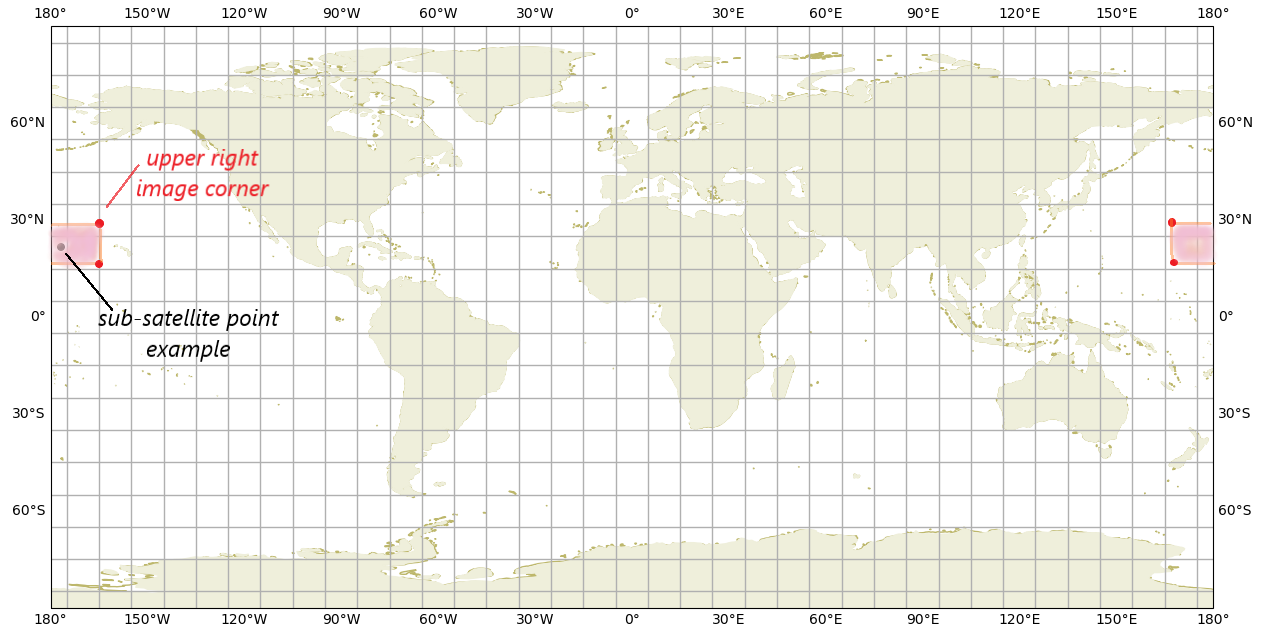
\includegraphics[width=0.9\textwidth]{Images/correct_calculation.png}\caption{Example of sub-satellite point on Earth and the four corners of the final captured image by its sensor. \textit{Source: Python code}}
\label{correct_calculation}
\end{figure}

\bigskip
\subsubsection{Tracking modification depending on sensor type}
\bigskip

One determinant parameter of the revisit time calculation is the swath width of the sensor as it was analyzed above. Nevertheless, the sensor type can change the final calculation. This is for example whether the instrument belongs to the passive or active imagery sensors (see section \ref{EO}). The reason behind is that when a satellite has passive instrument on board, it needs to be on the sunlit side of the Earth since those sensors record the reflected solar energy. Most of the EO satellites today are in near-polar sun-synchronous orbits, which have the following characteristic. \cite{Kramer 2002} The descending pass of the satellite, which is when the satellite travels southwards, is usually on the sunlit side in the case of a sun-synchronous orbit.

This application, therefore, checks whether the satellite has a passive sensor or not, and in case it has, the revisit time is calculated only for the descending passes of the satellite. In the Figure \ref{ascending-descending}, one orbit of the Sentinel-2A is shown; since it is a sun-synchronous orbit, the descending pass is on the sunlit side of the Earth and the ascending on the shadowed.

\begin{figure}
\centering
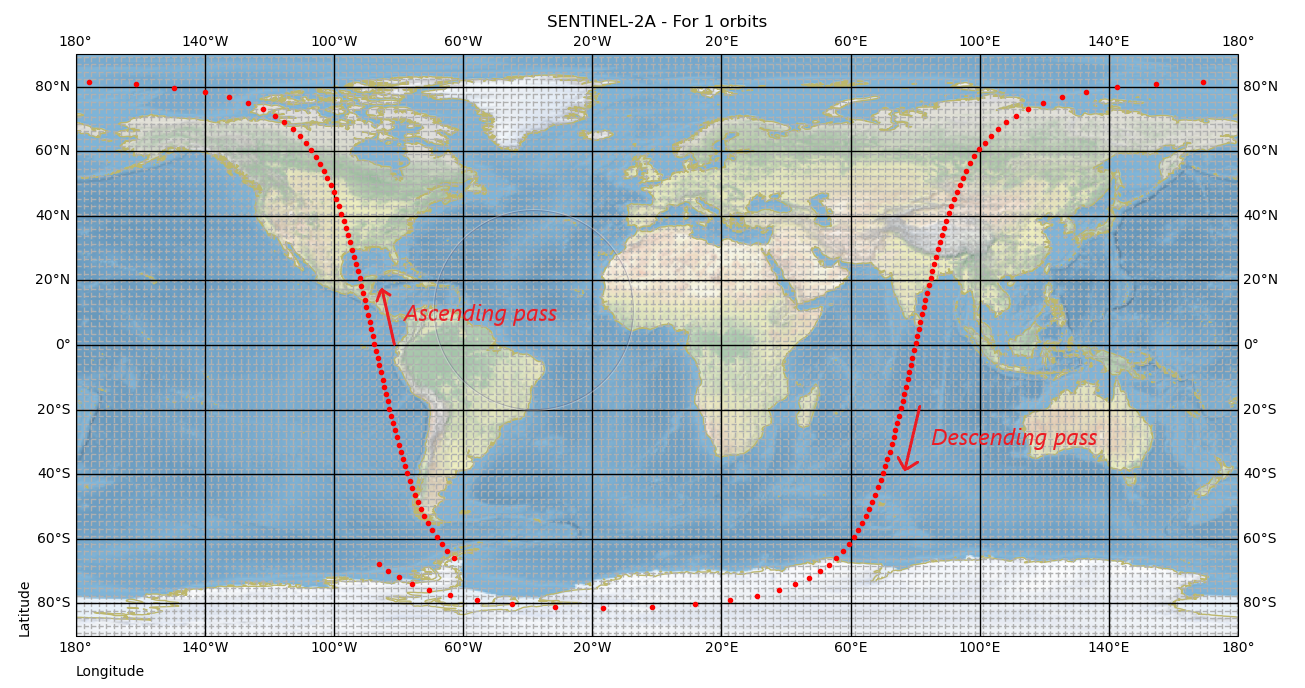
\includegraphics[width=0.9\textwidth]{Images/ascending-descending.png}\caption{The groundtrack of Sentinel-2A orbiting once the Earth. The ascending and descending pass can also be seen. \textit{Source: Python code}}
\label{ascending-descending}
\end{figure}

Yet another parameter that can change the calculation of the revisit time is whether the instrument has a nadir or titled looking sensor (see Figures \ref{nadir_looking} and \ref{tilted_looking}). In case a sensor has a titled looking capability, the result of the revisit time will not change, since all the counting of the cells will be shifted according to the respective tilt angle. However, if the information about the viewing geometry of the sensor is available, then the calculation of the revisit time can be actualized having taken into account this parameter as well.

\begin{figure}
\centering
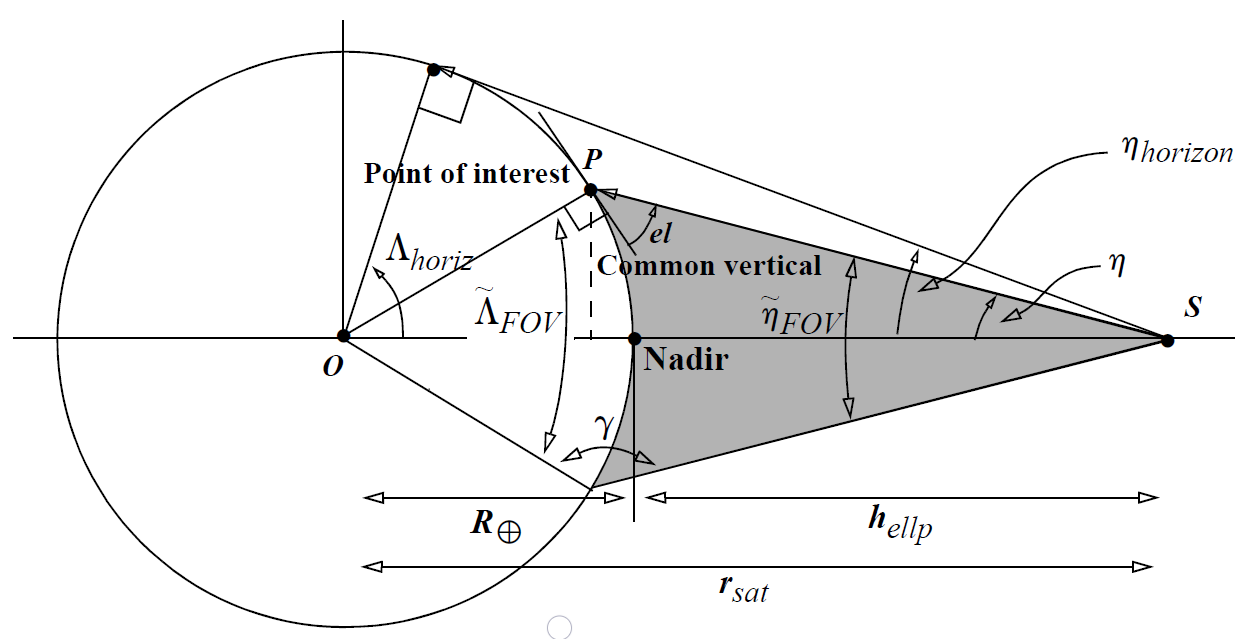
\includegraphics[width=0.9\textwidth]{Images/nadir_looking.png}\caption{An illustration of a nadir looking sensor. The satellite ($S$) is directly beneath the nadir point. Regarding the rest of the symbols: $P$ depicts the point of interest, $h_{\text{ellp}}$ the altitude of the ellipse, $\eta_{\text{FOV}}$ the boresight angle of the field of view, and $\Lambda$ the ground range. \textit{Source: modified \cite{Vallado}}}
\label{nadir_looking}
\end{figure}

\begin{figure}
\centering
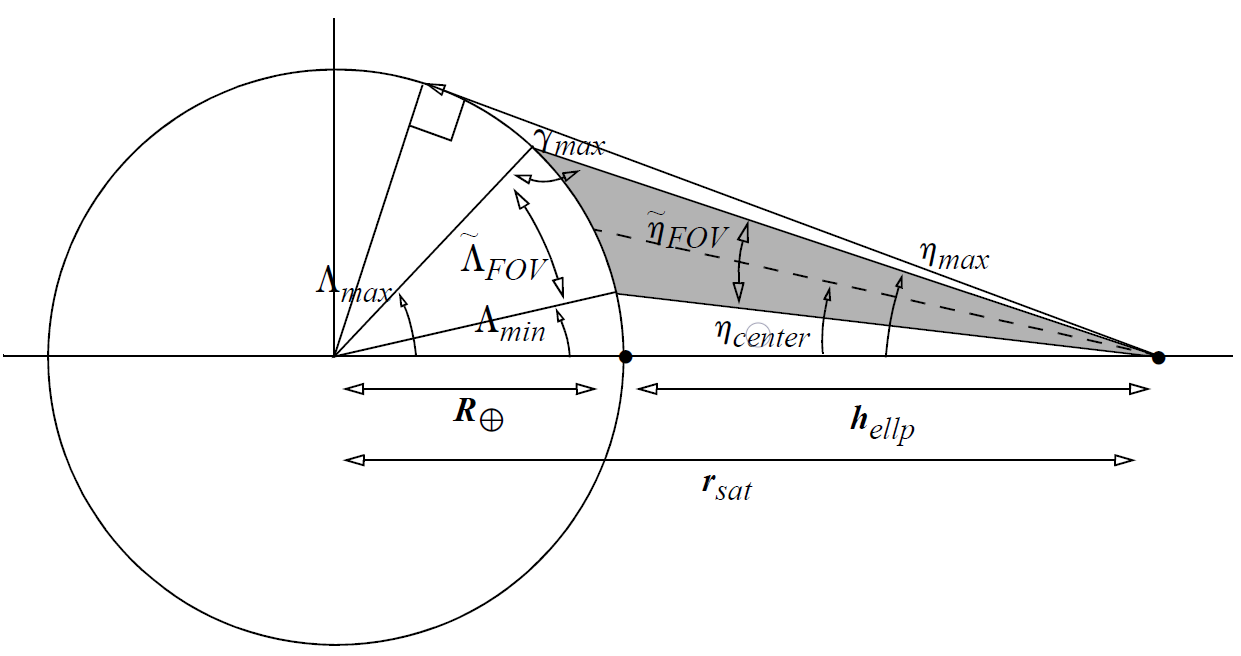
\includegraphics[width=0.9\textwidth]{Images/tilted_looking.png}\caption{An illustration of a titled looking sensor. The $\eta_{\text{center}}$ depicts the tilt angle. Regarding the rest of the symbols, see Figure \ref{nadir_looking}. \textit{Source: modified \cite{Vallado}}}
\label{tilted_looking}
\end{figure}

\bigskip
\subsubsection{Additional functions of the application}
\bigskip
The user has the option of selecting a certain latitude, in which he/she is interested in knowing the revisit time. Then, the above explained procedure of the calculation of the revisit time is followed again for the requested latitude. As already mentioned, the default option is the calculation of the revisit time at the equator.

Another capability of this application is that the revisit time in any latitude of not only one satellite, but of a constellation can be found. This means that the added value of the dozens of new satellites that are added to big EO constellations can be investigated.

\bigskip
The python code can be found in the appendices part (Section \ref{app}).

\bigskip
\section{Added value of satellite based on operational similar objects}
\label{added value}
\bigskip

The second capability of the application is to provide the user with the information about the current state of the LEO region in the field of EO satellites. More specifically, according to the user's request, the application parses, analyzes or calculates the orbital characteristics and attributes of the EO satellites that have been analyzed previously by the application (see section \ref{revisit time}) based on the input parameters that were imported by the user. Some real examples are presented in the next chapter.

\bigskip
\subsection{Database}
\bigskip

For the actualization of this goal, the creation of a database is necessary. In this way, there will be a system, in which all the information related to EO satellites orbiting in the LEO region can be stored along with the results obtained from the application that was previously described. Then, not only a user can benefit by finding out what is the added value of a future satellite based on how many other similar objects offer this service already, but also this database can be the springboard to new research studies related to the space traffic management rules. These rules need to be implemented based on the orbit and capacity allocation.

\bigskip
The database was implemented in \textit{PostgreSQL}, which is an open-source relational database management system with great capabilities.  

The main table that was created contains the keplerian elements of an orbit, which can be found in the TLE set of a satellite. Additionally, the parameters related to the EO sensors and instruments are also added (see section \ref{input_data}). In a nutshell, the added elements are the following: the unique international designator of a satellite, its name, the epoch, inclination ($i$), RAAN ($\Omega$), eccentricity ($e$), argument of perigee ($\omega$), mean anomaly ($M$), mean motion ($n$), the date of the launch, orbit lifetime, the name of the sensors on board, swath width, spatial resolution, and the type of instrument, whether it is an active or passive sensor.

The information that is also plugged in to the table is the satellite's revisit time in the equator. In order to be actualized, the application that was described in the section \ref{revisit time} runs having as input data, the information of this table. Then, the result of the application, which is the revisit time, is imported as a new information to the database.

\bigskip
\subsubsection{Sources of data}
\bigskip

The sources of the data are numerous. For this reason, another table containing this information was created. This is necessary in the case of an update in the information or when a parameter needs to be checked. Some of the most frequent references regarding the TLE set is the \textit{CelesTrak} from \textit{NORAD} and the \textit{Space-track.org} webpages. There are also multiple databases, which include in their records relevant to this application data.

\bigskip
\subsection{Classification of Earth Observation field}
\bigskip

It has been noticed that in the existed databases, it has not be made a classification of the Earth Observation field. This lack of distinction between the EO missions makes the search of added value of a satellite even harder. This happens due to the fact that the main objective of the mission is missing as an information from the existing databases. For this reason, a classification of EO field was made.

The categorization of the EO field is consisted of two main layers. The first one, which is the most general, refers to the source of funding of the mission as well as to the target group, which will use the satellite's output. So, in this layer the options are either commercial, research, defense, or civil (Figure \ref{classification_1st_layer}).

\begin{figure}
\centering
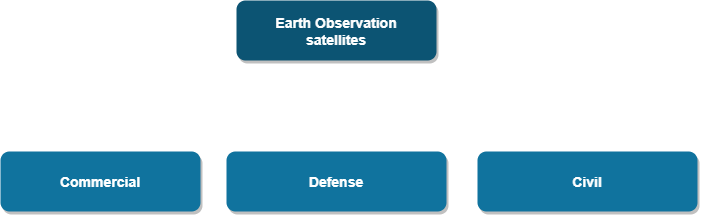
\includegraphics[width=0.9\textwidth]{Images/classification_1st_layer.png}\caption{The first layer of the classification of the field of Earth Observation.}
\label{classification_1st_layer}
\end{figure}

The second layer refers to the main objective of the mission. This can be related to environmental monitoring, emergency management, science, or security. These two aforementioned layers are not interconnected. This means that a satellite can have attributes with any possible combination of those. The rest of the layers are connected to the second one as it can be seen in Figure \ref{classification_2nd_layer}. In other words, from the main objective of a mission (second layer), a more explanatory and detailed description of the mission's goal is given in those labels.

\begin{figure}
\centering
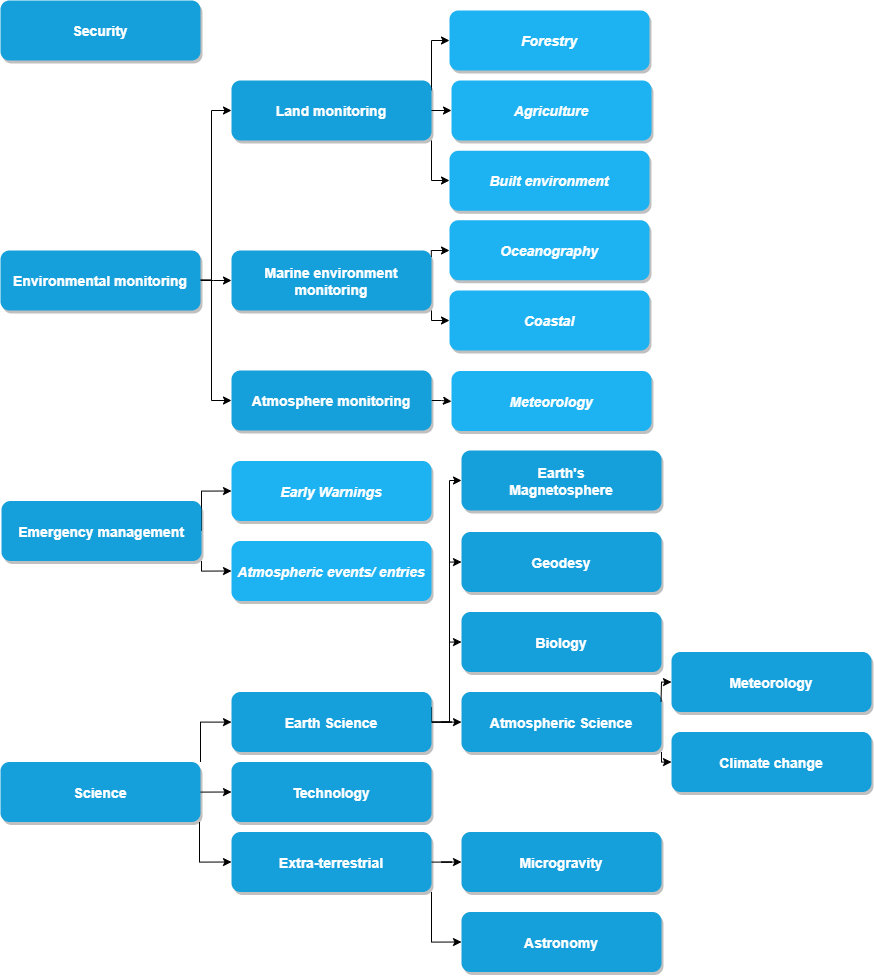
\includegraphics[width=0.9\textwidth]{Images/classification_2nd_layer.png}\caption{The second layer of the EO classification together with its further sub-categories.}
\label{classification_2nd_layer}
\end{figure}

This classification was implemented by taking into account various mission objectives and characteristics that were found in \cite{Newspace} and other databases, as it is mentioned in the previous section. Another source of influence was the work of Kramer [2002] \cite{Kramer 2002}. All in all, the creation of an objective, accurate, general and at the same time specific classification is a project that can have many solutions.

\bigskip
\subsection{Data import to the database}
\bigskip

The application as it was described at the beginning of this chapter together with the advantages and capabilities that a database brings, create a useful tool. This can be further improved by inserting more data to the database.

There are three possible ways of importing data in the database. The first one is through the server of the PostgreSQL locally, or in other words via the SQL application. The second one is through a configuration file (.ini file). In this way, the application first examines whether the imported satellite already exists in the database, or there is just a missing information regarding its revisit time, and then according to the answer it inserts it or not. The three way of importing data is from through a python script (see section \ref{app}), which is an automated process of inserting the TLE elements in the database.

\bigskip
The tables of the created database can be found in the appendices part (section \ref{app}).